\documentclass[12pt,a4paper]{article}
\usepackage[utf8]{inputenc}
\usepackage[spanish]{babel}
\usepackage{geometry}
\geometry{a4paper, margin=2.5cm}
\usepackage{hyperref}
\usepackage{graphicx}
\usepackage{tabularx}
\usepackage{titlesec}
\usepackage{float}

\title{\textbf{Análisis Reto: Primer Bimestre} \\ Sistema de Gestión de Pedidos e Inventario en Tiempo Real (ISBEN-B2B)}
\author{Alex Santiago Serrano Saca}
\date{\today}

\begin{document}

\maketitle
\tableofcontents
\newpage

\section{Capítulo 1: Introducción y Problemática}

\subsection{Introducción}
El presente documento detalla la fase de análisis y planificación del proyecto ISBEN-B2B, una plataforma web de intermediación mayorista. El sistema busca digitalizar y automatizar las ventas al por mayor mediante la validación de inventario en tiempo real, conectando a empresas distribuidoras, vendedores freelance y dueños de micromercados.

\subsection{Problemática}
La falta de sincronización en tiempo real del inventario genera altos costos logísticos para las empresas, ya que los vendedores físicos levantan pedidos a ciegas, ofreciendo productos agotados. Adicionalmente, los clientes finales (tenderos) se enfrentan a una brecha tecnológica que dificulta su abastecimiento autónomo, generando demoras en la cadena de distribución.

\subsection{Metodología o estrategia de desarrollo}
Se utilizará una metodología ágil (Scrum) estructurada en Sprints, enfocada en un desarrollo web a medida utilizando arquitecturas modernas (como MERN stack o similar) para asegurar la capacidad de sincronización de microservicios. Se descartan soluciones prefabricadas (como CMS) debido a la complejidad de las integraciones API y la concurrencia de la base de datos.

\section{Capítulo 2: Planificación y análisis}

\subsection{Análisis (Paso 1: Extracción de necesidades y objetivos)}
El análisis contempla el desarrollo de un módulo de gestión empresarial para catálogos, un sistema de evaluación de vendedores freelance, y una interfaz de compras ultra simplificada para los tenderos. Para derivar los requerimientos, primero se extrajeron las necesidades clave del documento de visión:

\begin{table}[H]
    \centering
    \begin{tabularx}{\textwidth}{|X|X|}
        \hline
        \textbf{Necesidad identificada} & \textbf{Fuente en el documento} \\ \hline
        Registro exclusivo de empresas y control de catálogos & Declaración del problema \\ \hline
        Proceso de pedido a prueba de errores para tenderos & Declaración del problema \\ \hline
        Sincronización de inventario exacta para evitar ventas fallidas & Enunciado de Visión \\ \hline
        Integración con software existente de las distribuidoras & Enunciado de Visión \\ \hline
        Exclusión absoluta de la plataforma en la facturación del producto & Restricciones Operativas \\ \hline
        Modelo de suscripción como única fuente de ingreso del sistema & Enunciado de Visión \\ \hline
    \end{tabularx}
    \caption{Extracción de necesidades operativas}
\end{table}

\subsection{Requisitos funcionales (Paso 2: Derivación)}
A partir de las necesidades extraídas, se definieron los siguientes requerimientos funcionales, asegurando su trazabilidad con los módulos correspondientes:

\begin{table}[H]
    \centering
    \begin{tabularx}{\textwidth}{|c|X|c|}
        \hline
        \textbf{ID} & \textbf{Descripción del Requerimiento Funcional} & \textbf{Trazabilidad} \\ \hline
        RF-01 & El sistema web permitirá el registro de empresas verificando datos legales básicos (RUC, Representante Legal) & M01-C01 \\ \hline
        RF-02 & El sistema permitirá a las empresas establecer límites mínimos de compra y gestionar el stock de su catálogo & M02-C01 \\ \hline
        RF-03 & El sistema habilitará el registro de vendedores freelance, incluyendo un módulo para rendir evaluaciones teóricas & M04-C01 \\ \hline
        RF-04 & El sistema web permitirá a tenderos y vendedores seleccionar productos y enviar un pedido formal a la empresa & M03-C01 \\ \hline
        RF-05 & El sistema verificará y descontará automáticamente el stock disponible en la base de datos al momento de confirmar un pedido & M02-C01 \\ \hline
        RF-06 & El sistema integrará una pasarela de pagos para procesar exclusivamente las suscripciones de las empresas a la plataforma & M01-C02 \\ \hline
        RF-07 & El sistema expondrá endpoints (APIs) seguros para recibir actualizaciones masivas de stock desde software contable externo & M05-C01 \\ \hline
    \end{tabularx}
    \caption{Derivación de Requerimientos Funcionales (RF)}
\end{table}

\subsection{Requisitos no funcionales (Paso 3: Derivación)}
Las restricciones de arquitectura, usabilidad y rendimiento se tradujeron en los siguientes requerimientos no funcionales:

\begin{table}[H]
    \centering
    \begin{tabularx}{\textwidth}{|c|X|c|}
        \hline
        \textbf{ID} & \textbf{Descripción del Requerimiento No Funcional} & \textbf{Trazabilidad} \\ \hline
        RNF-01 & La interfaz web debe ser desarrollada garantizando usabilidad extrema, con tipografías legibles y procesos guiados paso a paso & RR-01, SA-01 \\ \hline
        RNF-02 & El tiempo de actualización del inventario visible en la web no debe superar los 2 segundos tras una compra confirmada & CE-01, OB-01 \\ \hline
        RNF-03 & La plataforma web debe ser responsiva, adaptándose perfectamente a pantallas de escritorio y teléfonos móviles & R-01 \\ \hline
        RNF-04 & La arquitectura de la base de datos no debe contemplar la generación de facturas tributarias vinculadas a los pedidos & R-03 \\ \hline
    \end{tabularx}
    \caption{Derivación de Requerimientos No Funcionales (RNF)}
\end{table}

\subsection{Historias de Usuario / Casos de Uso}
\begin{itemize}
    \item \textbf{HU-01:} Como Tendero, quiero realizar pedidos desde una interfaz simple para abastecer mi local sin intermediarios físicos.
    \item \textbf{HU-02:} Como Empresa, quiero sincronizar mi inventario mediante una API para evitar vender productos sin stock.
    \item \textbf{HU-03:} Como Vendedor Freelance, quiero rendir una evaluación teórica dentro de la plataforma para obtener la aprobación de la empresa y empezar a levantar pedidos en físico.
    \item \textbf{HU-04:} Como Empresa, quiero pagar mi suscripción a través de una pasarela integrada para mantener activo el acceso al sistema y la visibilidad de mi catálogo de productos.
\end{itemize}

\subsection{Sprint}
El \textbf{Sprint 1} tendrá una duración de dos semanas y se enfocará en el diseño lógico de la base de datos, la configuración del repositorio y el desarrollo de los módulos de autenticación y validación de empresas (RF-01).

\subsection{Diagramas: Clases y BD (diseño lógico) - Preguntas y respuesta al diagrama}

\begin{figure}[H]
    \centering
    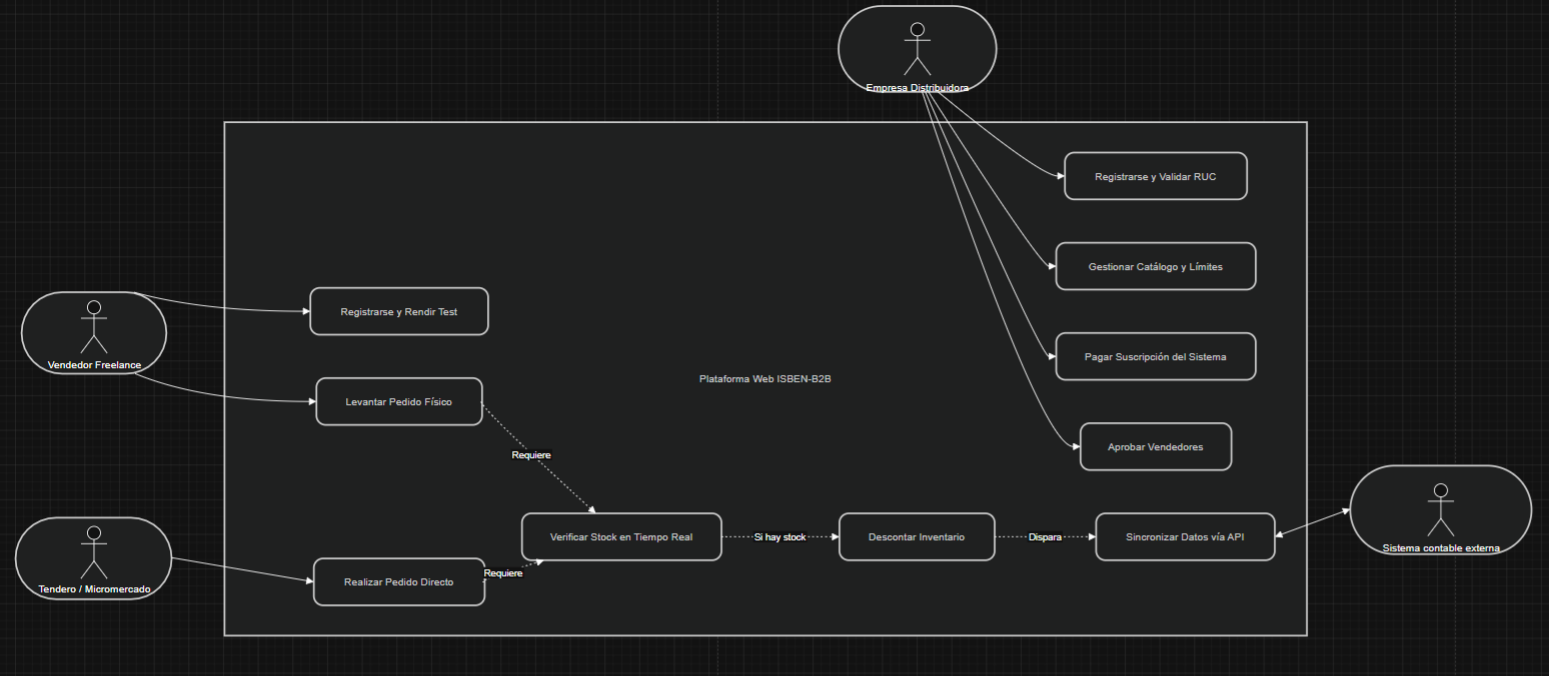
\includegraphics[width=0.9\textwidth]{DiagramasCasoUso.png}
    \caption{Diagrama de Casos de Uso para ISBEN-B2B}
\end{figure}

\begin{figure}[H]
    \centering
    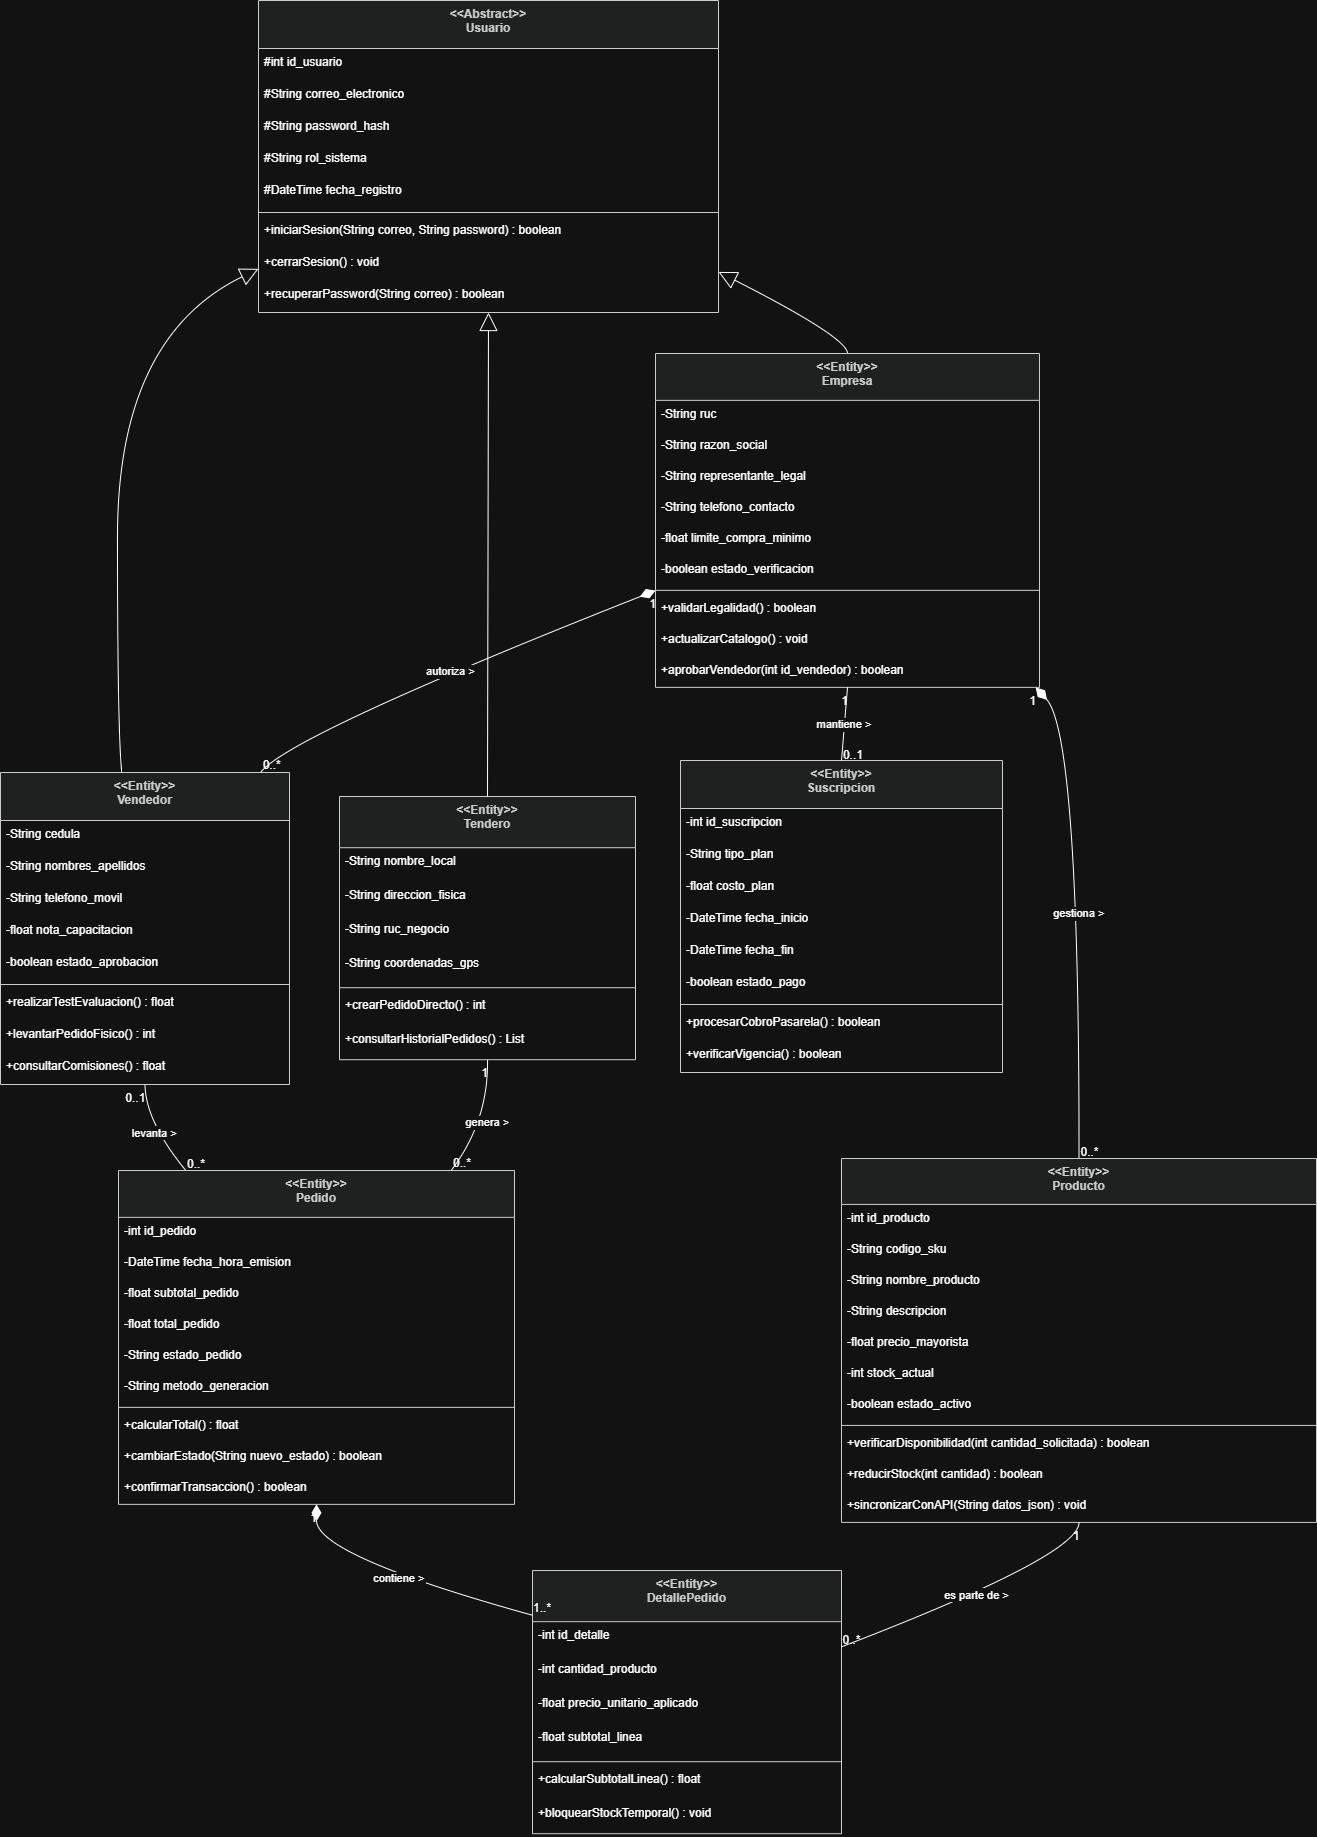
\includegraphics[width=0.9\textwidth]{DiagramaClases.png}
    \caption{Diagrama de Clases (Arquitectura Lógica) para ISBEN-B2B}
\end{figure}

\vspace{0.5cm}
\textbf{Preguntas y respuestas sobre el Diagrama de Clases:}
\begin{enumerate}
    \item \textbf{¿Por qué Empresa, Vendedor y Tendero heredan de la clase Usuario?} \\
    Para centralizar atributos comunes (correo, contraseña) y gestionar la autenticación en una sola entidad, evitando redundancia de código.
    \item \textbf{¿Cómo se garantiza el descuento correcto del stock?} \\
    Mediante la clase \textit{DetallePedido}, que verifica el stock del producto específico antes de confirmarse.
    \item \textbf{¿Qué relación hay entre Empresa y Suscripcion?} \\
    Una relación de 1 a 0..1, ya que la plataforma se monetiza mediante planes corporativos y una empresa puede no tener un plan activo en un momento dado.
    \item \textbf{¿Por qué sincronizarConAPI() está en Producto?} \\
    Para encapsular la lógica, asegurando que las actualizaciones del software contable afecten únicamente la disponibilidad e información del ítem.
    \item \textbf{¿Cómo modela el diagrama el inicio de la orden?} \\
    Tendero y Vendedor tienen asociaciones independientes hacia la entidad \textit{Pedido}, permitiendo rastrear el origen de la transacción.
\end{enumerate}

\subsection{Diagrama de componentes}
El sistema se compone de tres módulos principales: un \textbf{Componente Frontend Web} (interfaz de usuario responsive), un \textbf{Componente Backend} (lógica de negocio y motor de suscripciones) y un \textbf{Componente de Base de Datos}. Adicionalmente, incluye un nodo de interfaz para comunicación con las APIs contables externas de las empresas.

\begin{figure}[H]
    \centering
    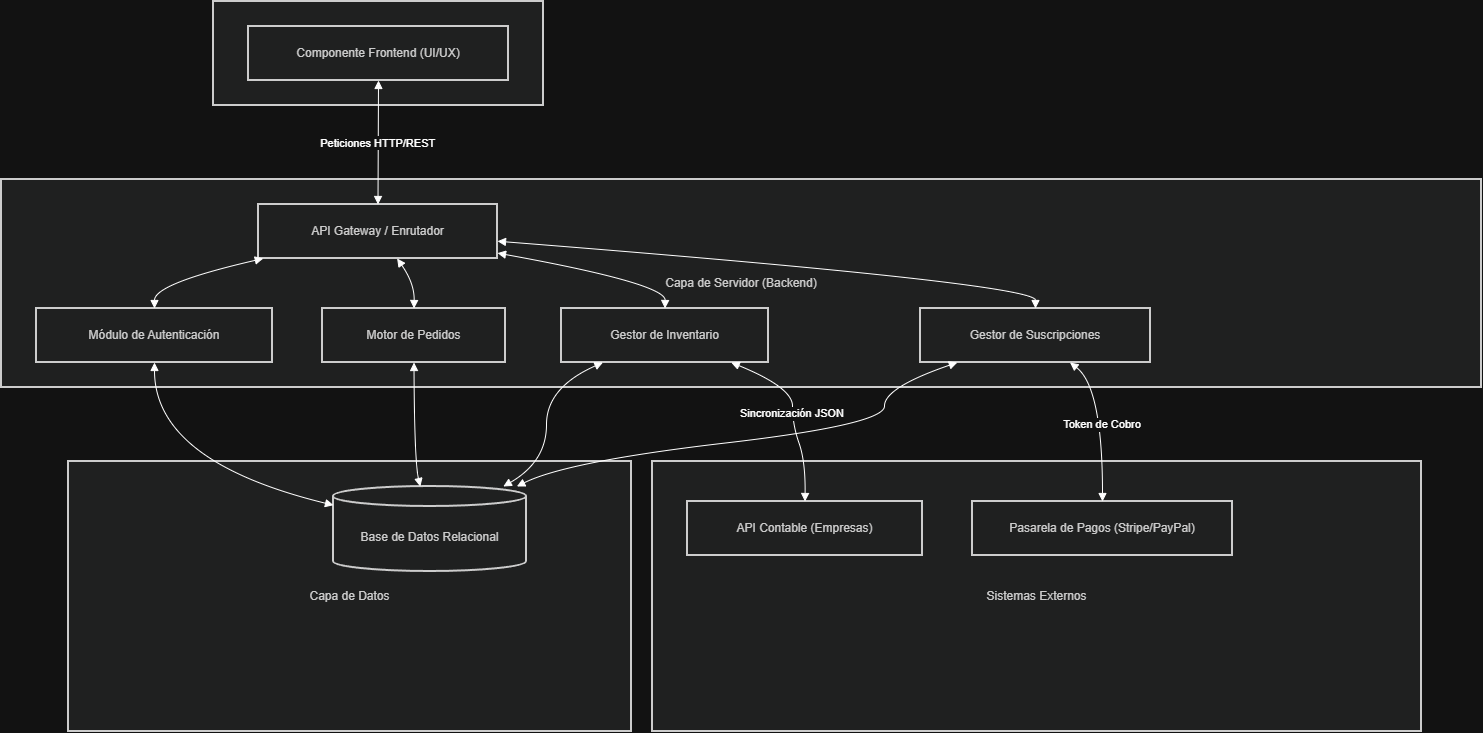
\includegraphics[width=0.95\textwidth]{DiagramaComponentes.png}
    \caption{Diagrama de Componentes del Sistema ISBEN-B2B}
\end{figure}

\subsection{Arquitectura lógica y física (propuesta)}
Se propone una arquitectura Cliente-Servidor alojada en la nube. Físicamente, el sistema constará de un servidor de aplicaciones para procesar las transacciones de pedidos y un servidor de base de datos relacional para garantizar la consistencia y transaccionalidad (ACID) del inventario cruzado.

\subsection{Prototipo de pantallas no funcional}
Se estructuraron wireframes de baja fidelidad donde destaca una navegación minimalista. Para la vista del Tendero, los prototipos omiten menús complejos, presentando únicamente barras de búsqueda amplias, botones de incremento de cantidad de tamaño grande y un resumen de pedido visible en un solo paso (checkout simplificado).

El prototipo interactivo web estructurado puede visualizarse y probarse en el siguiente enlace: \\
\url{https://attached-assets--ilynn1.replit.app/}

\end{document}